\documentclass[11pt]{LaTeX-Classes/math-hw}
\usepackage{float}
\usepackage{dirtytalk}
\title{Final Project: Computer Controlled Laser Engraver}
\firstname{Nicholas Hedges and  Wyatt Wayman}
\lastname{}
\coursename{ECE 3710 Fall 2020}
\professorname{Dr. Phillips}
\date{15 December 2020}

\begin{document}
\maketitle

\section{Introduction}
For our final project in ECE 3710, we are using our microcontroller and a PC to implement a 2D laser engraver. To do this, we developed code to scan an image file and break the image down into motor and laser instructions. Following this, the PC would send these instructions serially to the microcontroller via USB. The microcontroller uses the UART to receive and parse the instructions so they can be turned into motor and laser commands. The result is a fully functional laser engraver.

\section{Scope}
This document presents an overview and precise details of the laser engraver design,
as well as the methods and results of functional tests.
This document focuses primarily on microcontroller and software topics,
omitting some details in electrical and mechanical design to save space.

\section{Design Overview}
This section covers an overview of our laser engraver design. This section will discuss the required functionality, the required components for building, the theory of operation, and the potential design alternatives. 
\subsection{Requirements}
Our laser engraver shall meet the following functionality requirements:
\subsubsection*{Hardware}
	\begin{itemize}
		\item The laser engraver shall etch at least a 80 mm by 80 mm square.
		\item The laser and x-y actuators shall be mounted within their own secure housing.
		\item The laser shall be securely attached to the x-y actuators.
		\item The laser brightness shall be changed for different instruction purposes.
		\item The microcontroller shall communicate serially with the PC via USB.
	\end{itemize}

\subsubsection*{Software}
	\begin{itemize}
		\item The laser location shall return to a home position with a single instruction.
		\item The PC software shall process image files to determine the necessary laser commands to create an image similar to that found in the image file.
		\item The microcontroller shall receive instructions manually through a terminal on the PC.
		\item The microcontroller shall receive instructions automatically from the PC via the image breakdown program.
		\item The microcontroller shall send a response flag via the UART back to the PC upon instruction completion.
		\item The microcontroller shall to send an error flag via the UART back to the PC upon invalid instruction.
	\end{itemize}

\subsection{Dependencies}
The following components are required to build the complete laser engraver design:
\begin{itemize}
	\item STM32 Microcontroller
	\item PC
	\item (2) X-Y linear actuators
	\item (2) MP6500 bipolar stepper motor drivers
	\item (2) Contact switches
	\item Mini USB cable
	\item 12V power supply
	\item NEJE 2.5W Laser Engraver Module Head 450nm 
	\item Included laser power board
	\item (4) Scrap plywood for laser engraver housing
	\item (4) Aluminum angle brackets
	\item (12) M3 machine screws
	\item (40) Wood screws
	\item (2) 2.2 kOhm resistors
	\item (2) Red LEDs
	\item Jumper wires as required
	\end{itemize}

\subsection{Theory of Operation}
The laser engraver operates on a number of principles to meet the end goal of
translating an image file on a computer to an image etched into wood or another material.

The PC has the responsibility of opening the image file and producing a list of commands to send to the microcontroller through the
USB connection. Once sent, the PC waits for a response indicating the command is complete
before sending the next one in the queue.

The microcontroller receives the commands through UART and parses the information to determine
what kind of command it is.  Once the command is determined, the parameters of the input are passed to the correct function.
These commands can be set by the software, or alternatively entered manually by the user
into a serial terminal software such as PuTTY.

The following are the laser engraver commands:
\begin{itemize}
  \item Home (no parameters)

    This command moves the actuators towards the top left hand corner until the homing switches
    are toggled, indicating that it can go no further.

  \item Goto (x destination, y destination)
    
    This command moves the actuators from their current location to the x and y coordinates
    as mapped onto the plane accessible to the actuators.

  \item Burn Horizontal (x destination, power output)

    This command starts at the current location and moves the laser to the right or left (negative number for left)
    while the laser is activated at a power level (between 0 and 999) specified.

  \item Burn Vertical (y destination, power output)
    
    Similar to Burn Horizontal, this command activates the laser as specified and moves the laser in the
    y direction.

  \item Burn Square (side length)

    This command moves the laser in a clockwise square, without changing the power level. It is
    mainly used for testing purposes.
\end{itemize}

The microcontroller uses state variables and parameter variables based on the command contents to determine which commands
to run and how long it should run them.

A timer causes synchronous processing of the state and parameters. Every 1 millisecond
the state variable is checked, as well as the current motor location, the target location,
the motor step state, the inputs from the homing switches, and any other relevant information.
The outputs to the actuator control lines are adjusted as necessary by toggling a step pin while
holding the corresponding direction pin high or low.
This causes the motors to navigate to their destination, as long as the state permits it.

If the command involved a burn, a different timer configured for Pulse Width Modulation is set
to the proper duty cycle based on the power parameter.

Once the command is complete, the UART sends a capital \say{A} followed by a newline
to indicate to the user or PC software that the command is complete.
If the command was a burn command, the laser is set to a very low duty cycle afterward. This prevents
burn spots from forming while the next command is being processed.

The end result of all these processes is that the inputted image is burned onto the material.

\subsection{Design Alternatives}
\subsubsection{Cheaper option: dual reflective mirrors}
A cheaper alternative concept was considered that consisted of a fixed laser and
mirrors mounted to already acquired stepper motors. The stepper motors would change the angle of the mirrors to reflect
the laser to the desired position. This idea was abandoned because of the distortion
that would be caused by the optical reflection and beam divergence problems.

\subsubsection{More involved option: CO$_2$ laser}
A high quality laser engraver and cutter could be made by using a very high power Carbon Dioxide-based
tube laser. This idea seemed ambitious and very involved, since the tube laser is much bigger
and would require a liquid cooling system.

\section{Design Details}
The laser engraver operates on a number of principles to meet the end goal of
translating an image file on a computer to an image etched into wood or another material.
We can follow the pipeline of information to see how it works.

\subsection{PC Software}
First, the image file on the computer is opened and read by the PC software using an open source
image processing library. The dimensions of the image are analyzed, and cropped to a smaller size
if necessary.
The image is converted to grayscale, and a preview is displayed to the user.
The software then scans through each pixel on the image, and builds groups of adjacent pixels
which have the same value. It generates a list of commands as it goes and they are queued in memory.
The list of commands, when executed in the right order, will tell the laser engraver how to make the image.

Once the user is ready, the software sends the first command, usually a \say{home} command, to the
microcontroller through the UART serial interface.
It waits for a response from the microcontroller, which is an indication that the command has been
carried out and the engraver is ready for a new command.
The second command is then sent, and the process repeats until all commands have been sent and executed.

\subsection{Microcontroller Software}
The microcontroller is key for the functionality of the overall system.
When the microcontroller (MC) is first powered on, it initializes all the necessary inputs and outputs,
which include pins for UART, inputs for switches, an analog output with the necessary timer,
and two output pins for each motor.
Additionally the sysTick timer is initialized. The overall operation of the MC is defined by some
state variables. Once everything is ready, the state is set to idling.

When data arrives through the UART interface, an interrupt is called by the hardware, and the
input is copied into a buffer. When a carriage return is received, indicating the end of a command,
the buffer is processed to read the name of the command and any included arguments.

The state machine and parameters such as the x and y destination coordinates are set.
The sysTick timer, which is always running, checks the state variables to determine what it should
do each time. For example, if it sees that the current state is GoTo, it should compare the current
motor locations and destinations to determine if the command is complete. Otherwise it should
determine which direction the motors need to move, and set the direction pin while toggling
the step pin on the motors as needed.

%TODO continue narrative

 \begin{figure}[H]
   \begin{center}
     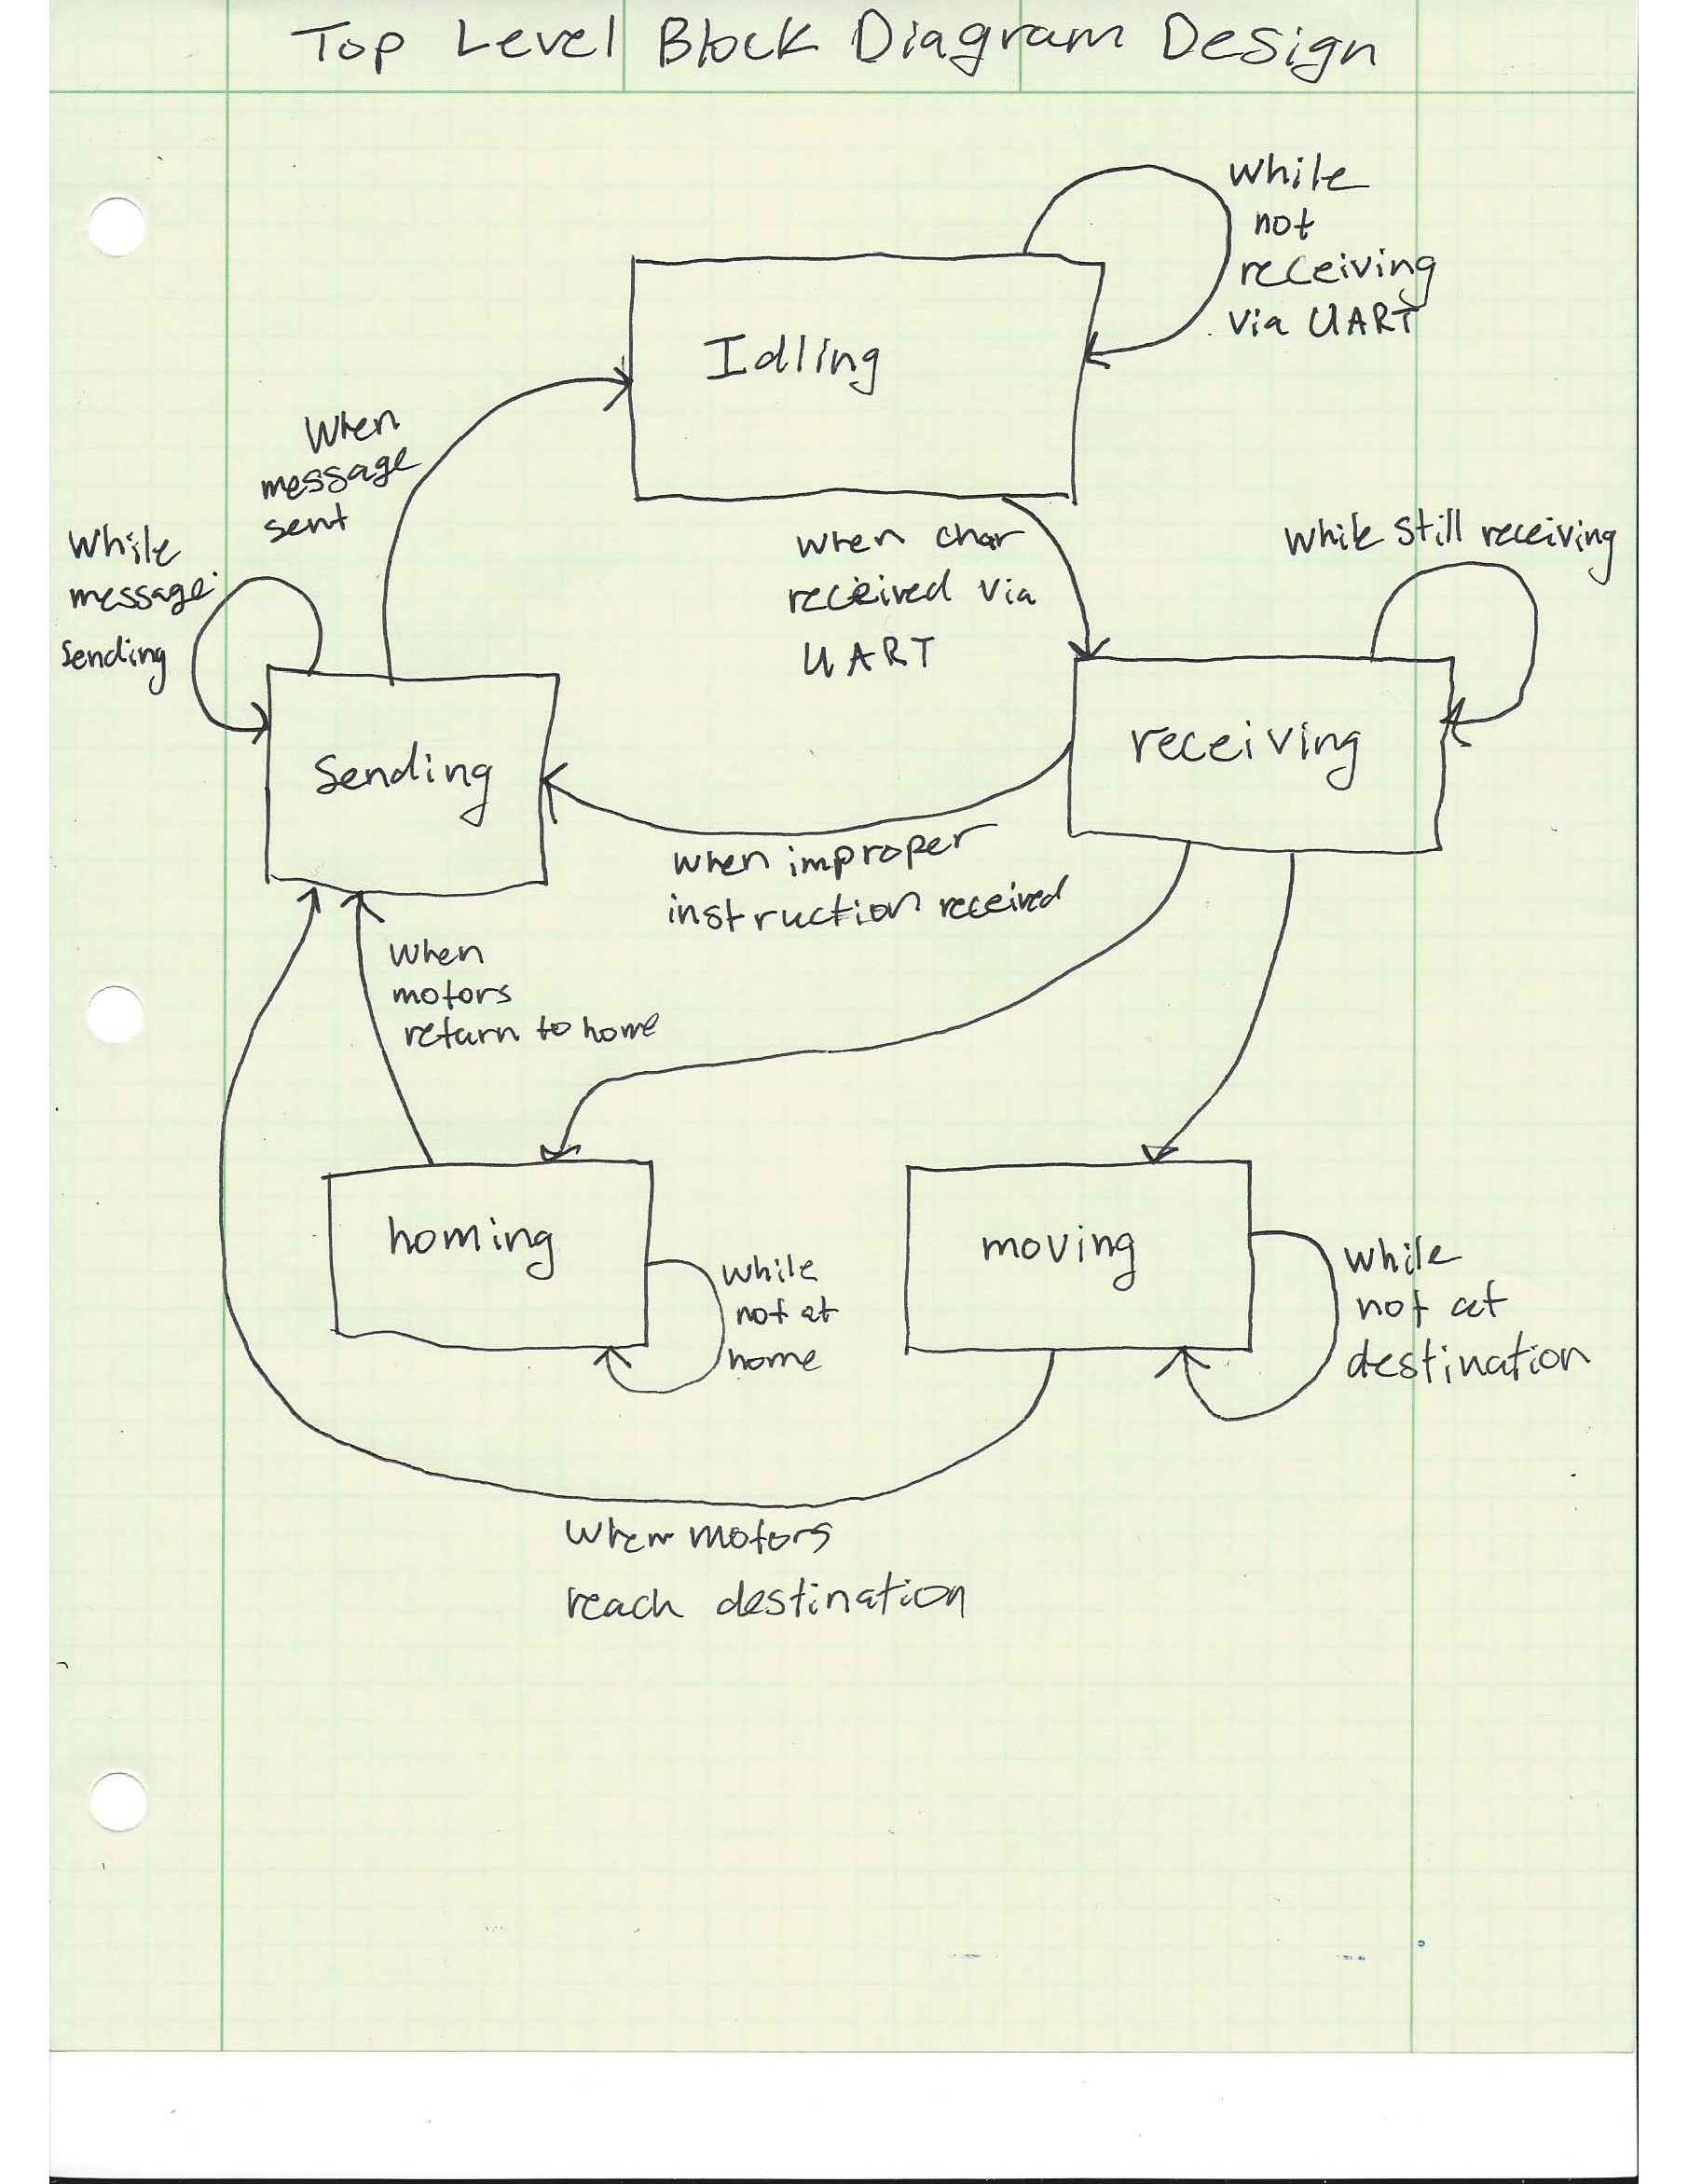
\includegraphics[width=0.6\textwidth]{blockdiagram}
     \caption{Top level design for the flow of states of our laser engraver}
     \label{fig:blockdiagram}
   \end{center}
 \end{figure}

\subsection{Electrical Hardware}

\begin{figure}[H]
	   \begin{center}
	     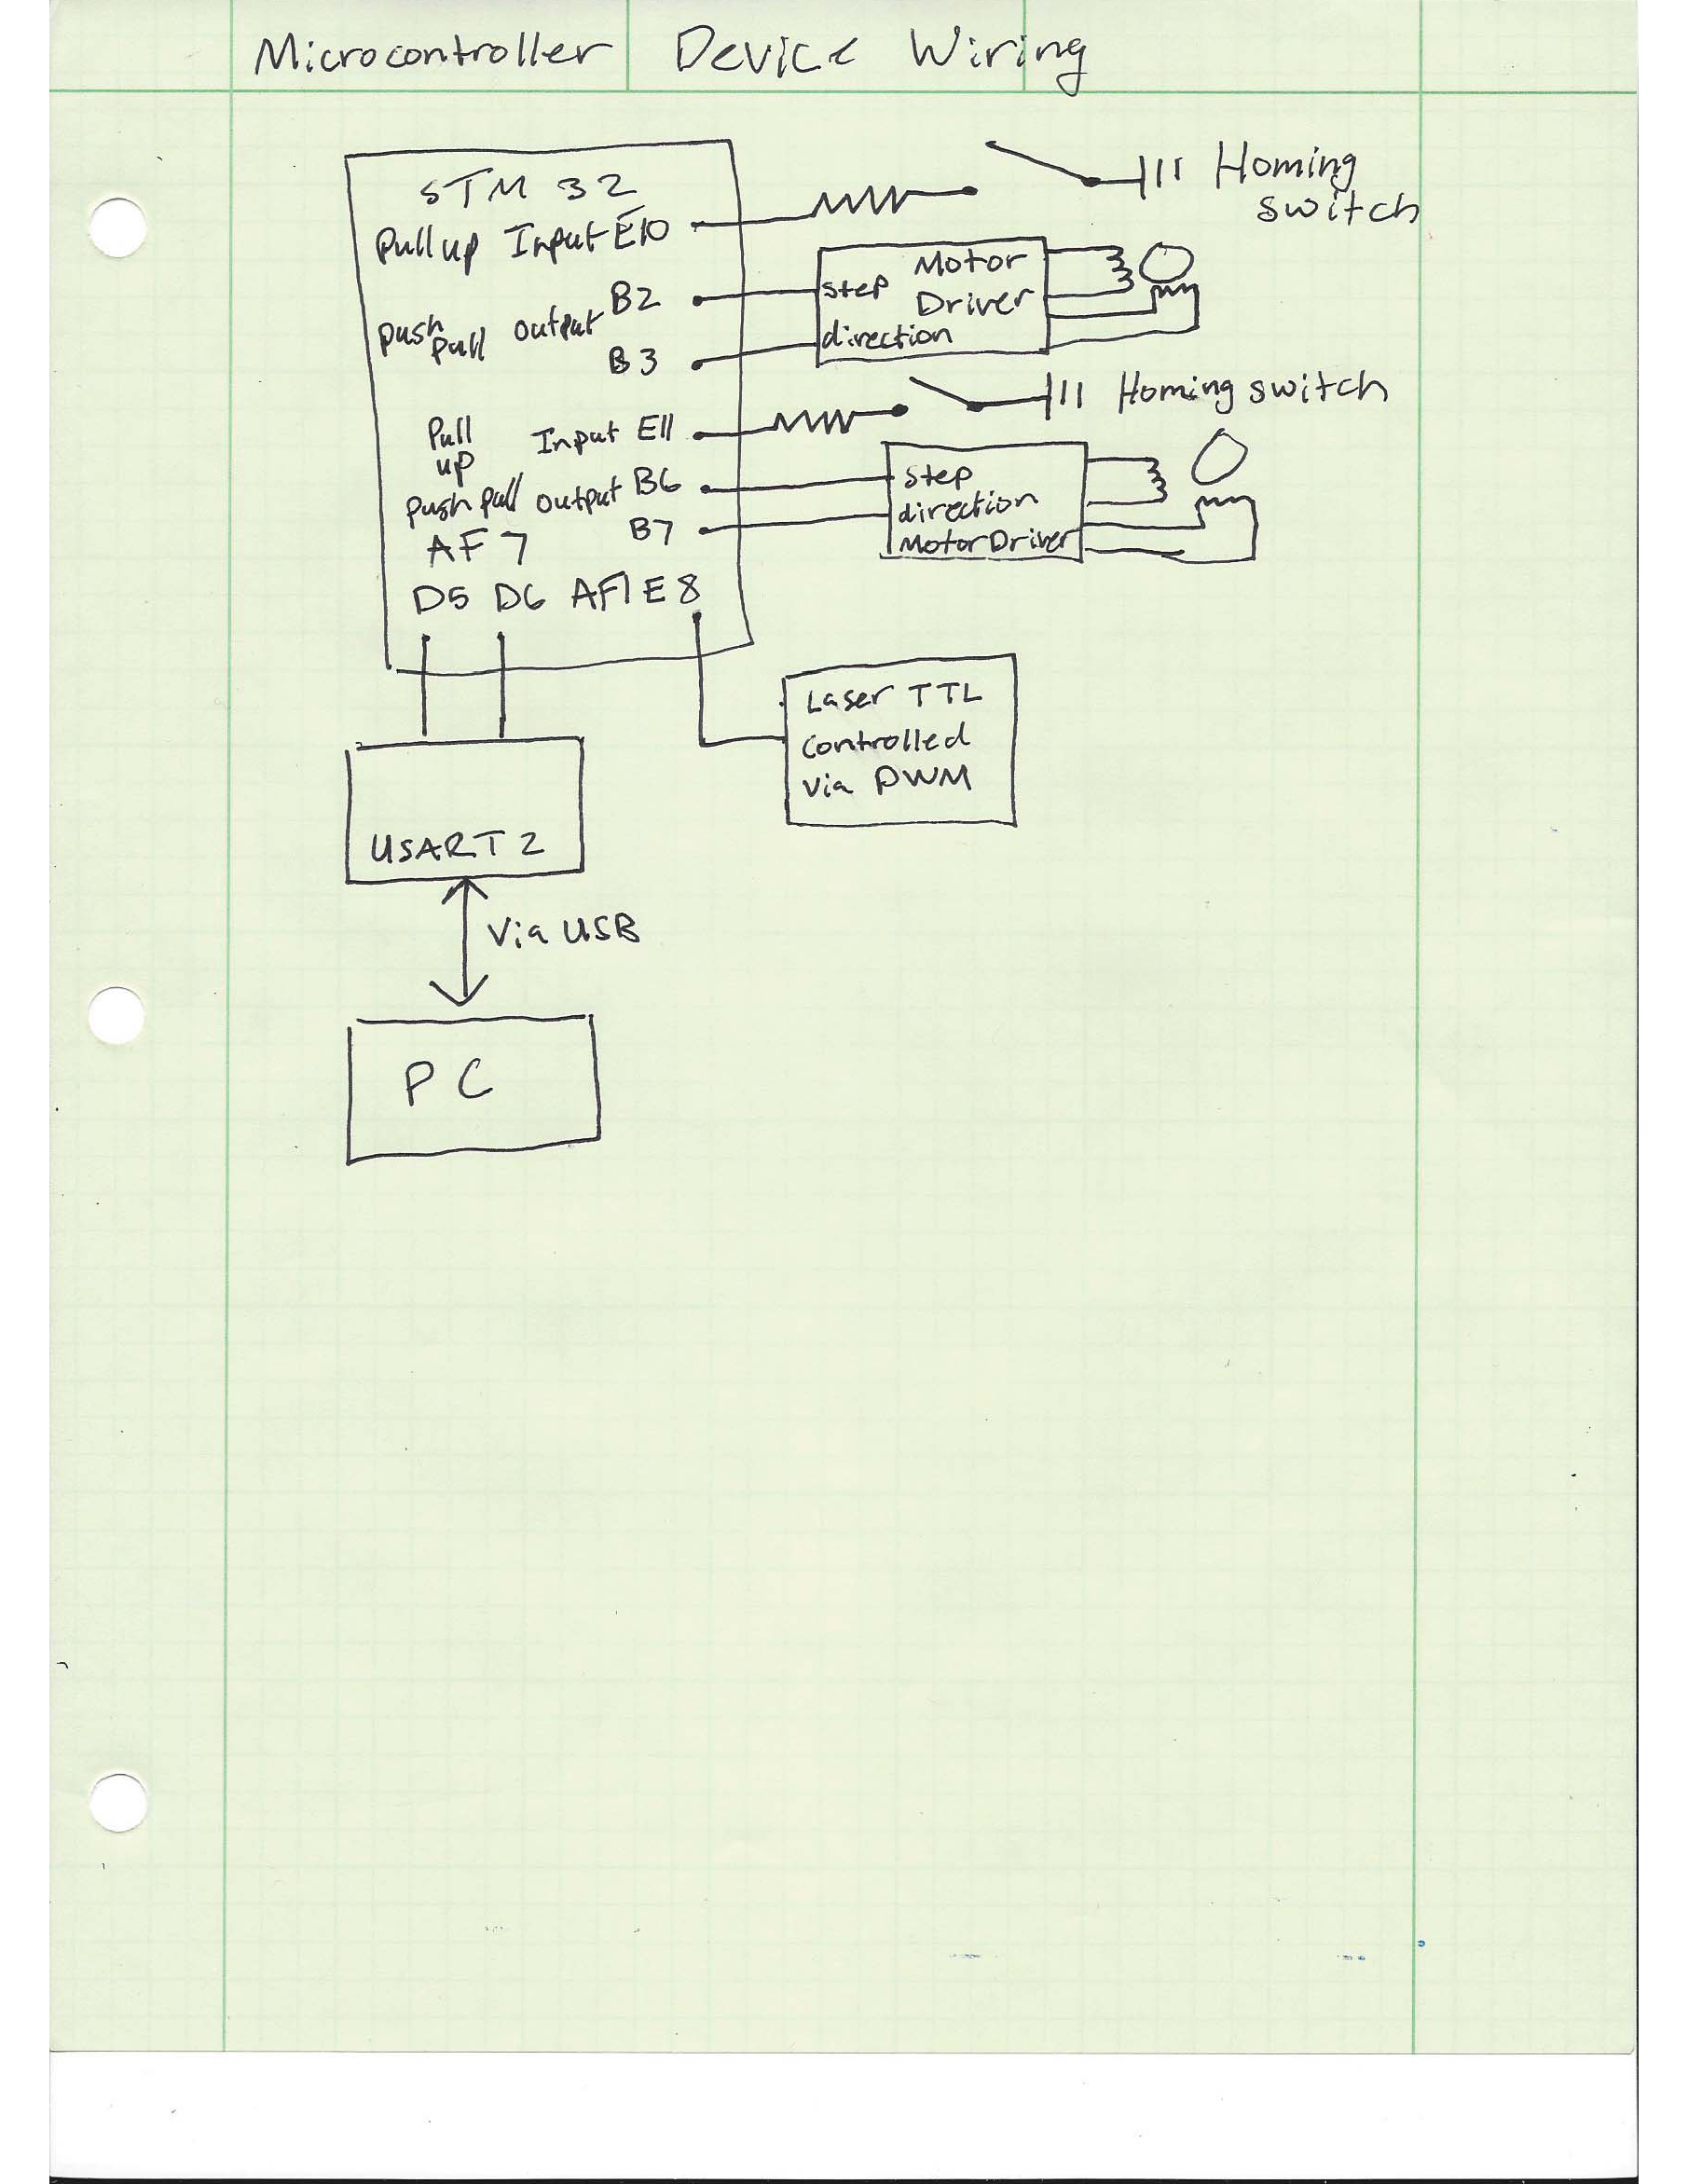
\includegraphics[width=0.6\textwidth]{mcwiringdiagram}
	     \caption{Top level design for the flow of interrupts and timers.}
	     \label{fig:mcwiringdiagram}
	   \end{center}
	 \end{figure}

\subsection{Mechanical and Wiring}

\section{Testing}
This section will go over the tests performed on our laser engraver to ensure it meets all of the functionality requirements. 

\subsection{Structure Test}
To begin the structure test, we visually examined the structure for any building imperfections and to ensure proper functionality could be achieved. Next, we used our hands to provide pressure on multiple sides of the housing to test for building security. From there we put light pressure on the x-y linear actuators to ensure they were securely fastened. Finally, we used a ruler to measure the size of the engraving area to ensure the size was large enough. From this test, we did not notice any visual design flaws and the structure seemed to be very sturdy. The etching area was determined to be 94 mm by 94 mm in size. This test was able to verify our laser engraver could etch a minimum of an 80 mm by 80 mm area, the housing for the laser and the motors were secure, and the laser and motors themselves were securely fastened.

\subsection{Motor Functionality Test}
This motor functionality test was performed by hard coding and running motor move commands from the microcontroller and observing the movement of the actuators afterward. We started by implementing move commands for each individual actuator to get them to move to the ends of their respective ranges. Following this, we implemented simultaneous move commands so both actuators would be moving at the same time. This test was performed to ensure the laser could be moved to any location within the etching area. We found that the actuators were able to move properly verified they could move at the same time. 

\subsection{Homing Test}
The homing test was conducted by hard coding and running move commands from the microcontroller to get the actuators to be in two non-zero locations. Next, a home command was hard coded and run to verify the laser would return to the 0,0 position. We observed that actuators went to the given location and were able to return back to the starting location via the home command. This test verified that the actuators can return to a home position with a single command.  

\subsection{Laser PWM Test}
The laser PWM test was performed by hard coding values into the microcontroller's timer one capture and control register to vary the PWM output for the laser. The values tested were from 99 to 999 in 100 unit increments. Once the value was loaded into the register, we would turn on the laser to observed its brightness. We observed that each value loaded into the capture and compare register adjusted the power level our laser outputted from a 90\% duty cycle down to a .1\% duty cycle. This test was able to verify our laser brightness can be changed for different instruction purposes.
 
\subsection{USB UART Communication Test}
The USB UART communication test was performed by connecting the microcontroller to a PC via a mini USB and disconnecting the laser and both actuators pins. Once connected, the PC sent commands serially to the microcontroller via a PuTTY terminal to ensure the microcontroller was receiving the commands and sending the proper response flag back to the terminal. We observed that all valid function calls were returned with the proper done flag and all invalid inputs were returned with the proper error flag. This test verified the microcontroller can communicate serially with the PC via USB and can send a done or error flag via the UART back to the PC upon instruction completion or failure.

\subsection{Image Instruction Breakdown Test}
The image instruction breakdown test was performed by configuring the software to print out
generated commands to the terminal. We observed test images could be loaded and when compared to the output of the program saw they were being
analyzed in a reasonable way. Figure \ref{fig:test-images} shows some example images that were used. This test verified the PC software can process image files to determine the necessary laser commands to create an image similar to that found in the image file.
\begin{figure}[H]
  \begin{center}
    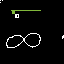
\includegraphics[width=0.4\textwidth]{test3}
    
\includegraphics[width=0.4\textwidth]{test4}
    \caption{Some images used to test the image breakdown}
    \label{fig:test-images}
  \end{center}
\end{figure}

\subsection{Manual Instruction Input Test}
The manual instruction input test was performed by connecting the microcontroller to a PC via a mini USB and connecting the laser and both actuators pins. Once connected, the PC sent commands serially to the microcontroller via a PuTTy terminal to ensure the microcontroller was receiving the commands and implementing the function calls correctly. We sent the following instructions: GO 5000, 5000; HM; GO 1000, 1000; BH 1000, 500; BV 1000, 500; GO 2000, 2000; SQ 1000, 500; and HM. We observed the actuators and the laser working as expected for each function call and also observed the done flag being sent back to the terminal on each successful instruction completion. This test verified the microcontroller can receive instructions manually through a terminal on the PC.

\subsection{Computer Generated Input Test}
The manual computer generated input test was performed with
the laser and motors were disconnected for convenience. This test was performed by
connecting the Linux PC to the microcontroller and using the image breakdown software to send the commands for
a known test image. It would skip the \say{home} command at the beginning and end since the motors
could not move.
We observed command completion acknowledgments were being consistently received after each instruction input.
This test verified the microcontroller can receive instructions automatically from the PC software.

\subsection{Full Functional Test}
The full process pipeline is tested by starting with an image file, loading it into the software,
and burning the image using the laser and motors automatically.
Test images were used first to verify that the image was consistently generated. We observed the laser engraved output matched closely to the inputted image. This test verified the microcontroller can receive instructions automatically from the PC via the image breakdown program.

\section{Conclusion}
The project overall was a success. There were some problems early on getting the actuators to work because we realized it was impossible to use the motor driver that came in our lab kits.
The x-y actuators were bipolar motors instead of unipolar motors, so they had no fifth wire or center tap to the coils. We ended up having to buy two bipolar stepper motor drivers to get the actuators working and that turned out successful.

Constructing the mechanical aspects of the device was more tedious than we had imagined,
but with some help and lots of time the chassis design was also realized. 

Collaborating remotely most of the time proved a challenge, but the use of git software allowed
relatively fast review and versioning of the code.

The end result is fairly impressive; a fully functioning system which meets all the requirements
and etches an image into wood or other materials.
The images seem to turn out OK. An example is shown in Figure \ref{fig:troll-print}.
\begin{figure}[H]
  \begin{center}
    
\includegraphics[width=0.4\textwidth]{trollface-edges}
    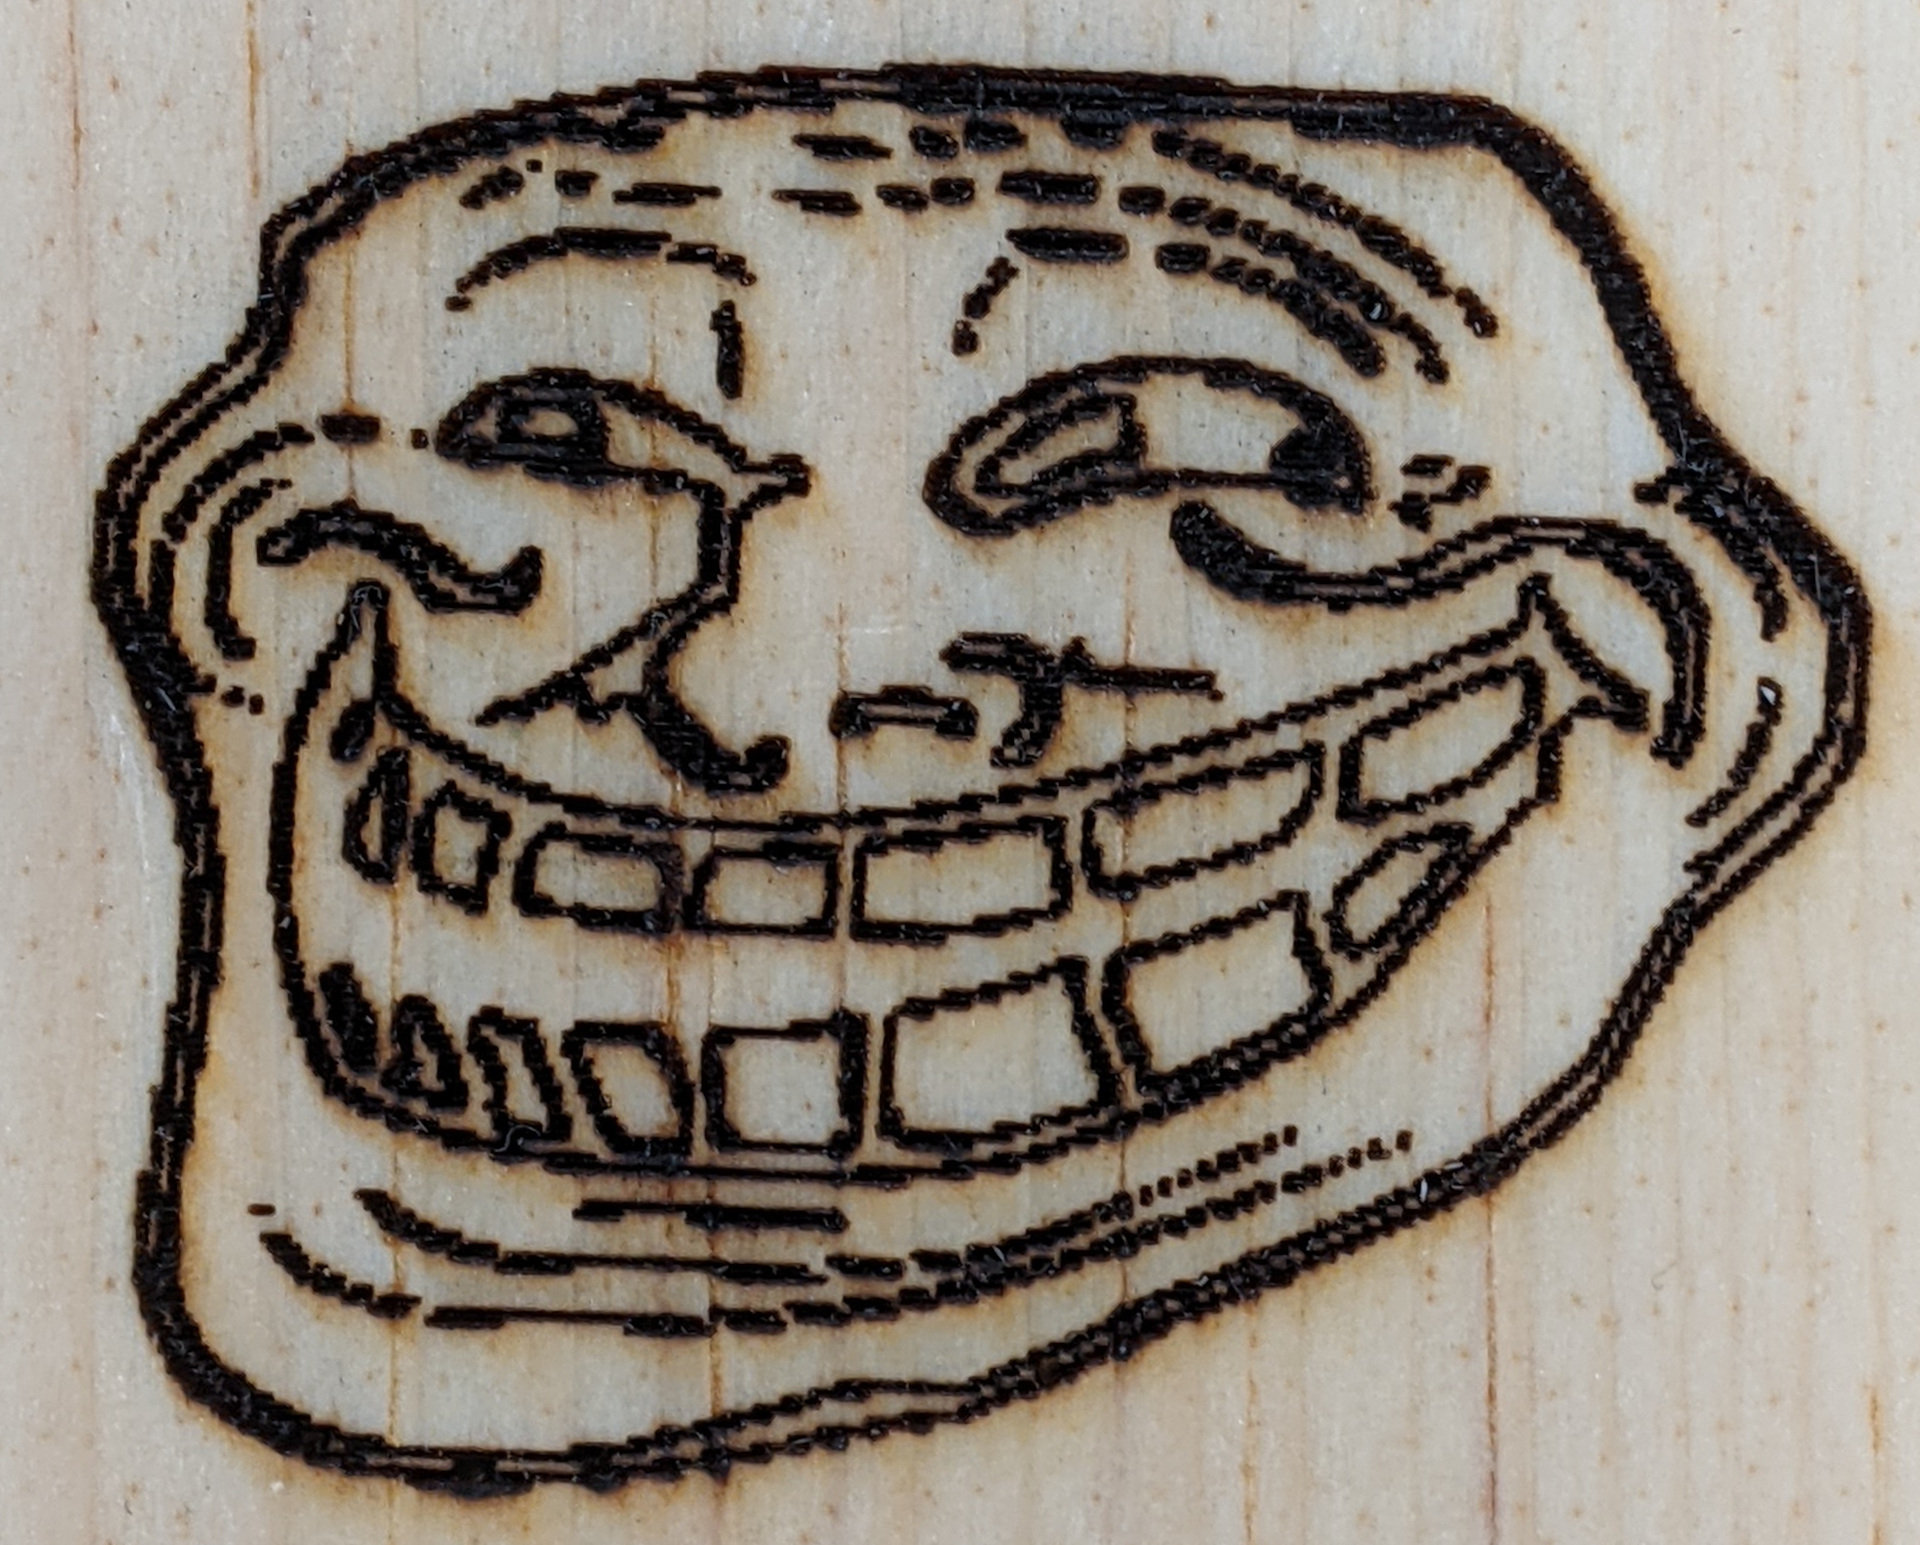
\includegraphics[width=0.4\textwidth]{trollface-result}
    \caption{The prepared input file and result in wood of an old internet meme}
    \label{fig:troll-print}
  \end{center}
\end{figure}

In Figure \ref{fig:burn-zoomed} we can see the way that the individual cuts were executed to
create the image.
Each numbered scale mark is one millimeter.
One thing that would be nice is if the mapping of the image was done differently.
This method requires lots of left and right scanning, which results in the rough, pixely edges
and the print taking a long time to execute- about an hour for a fairly small image.
\begin{figure}[H]
  \begin{center}
    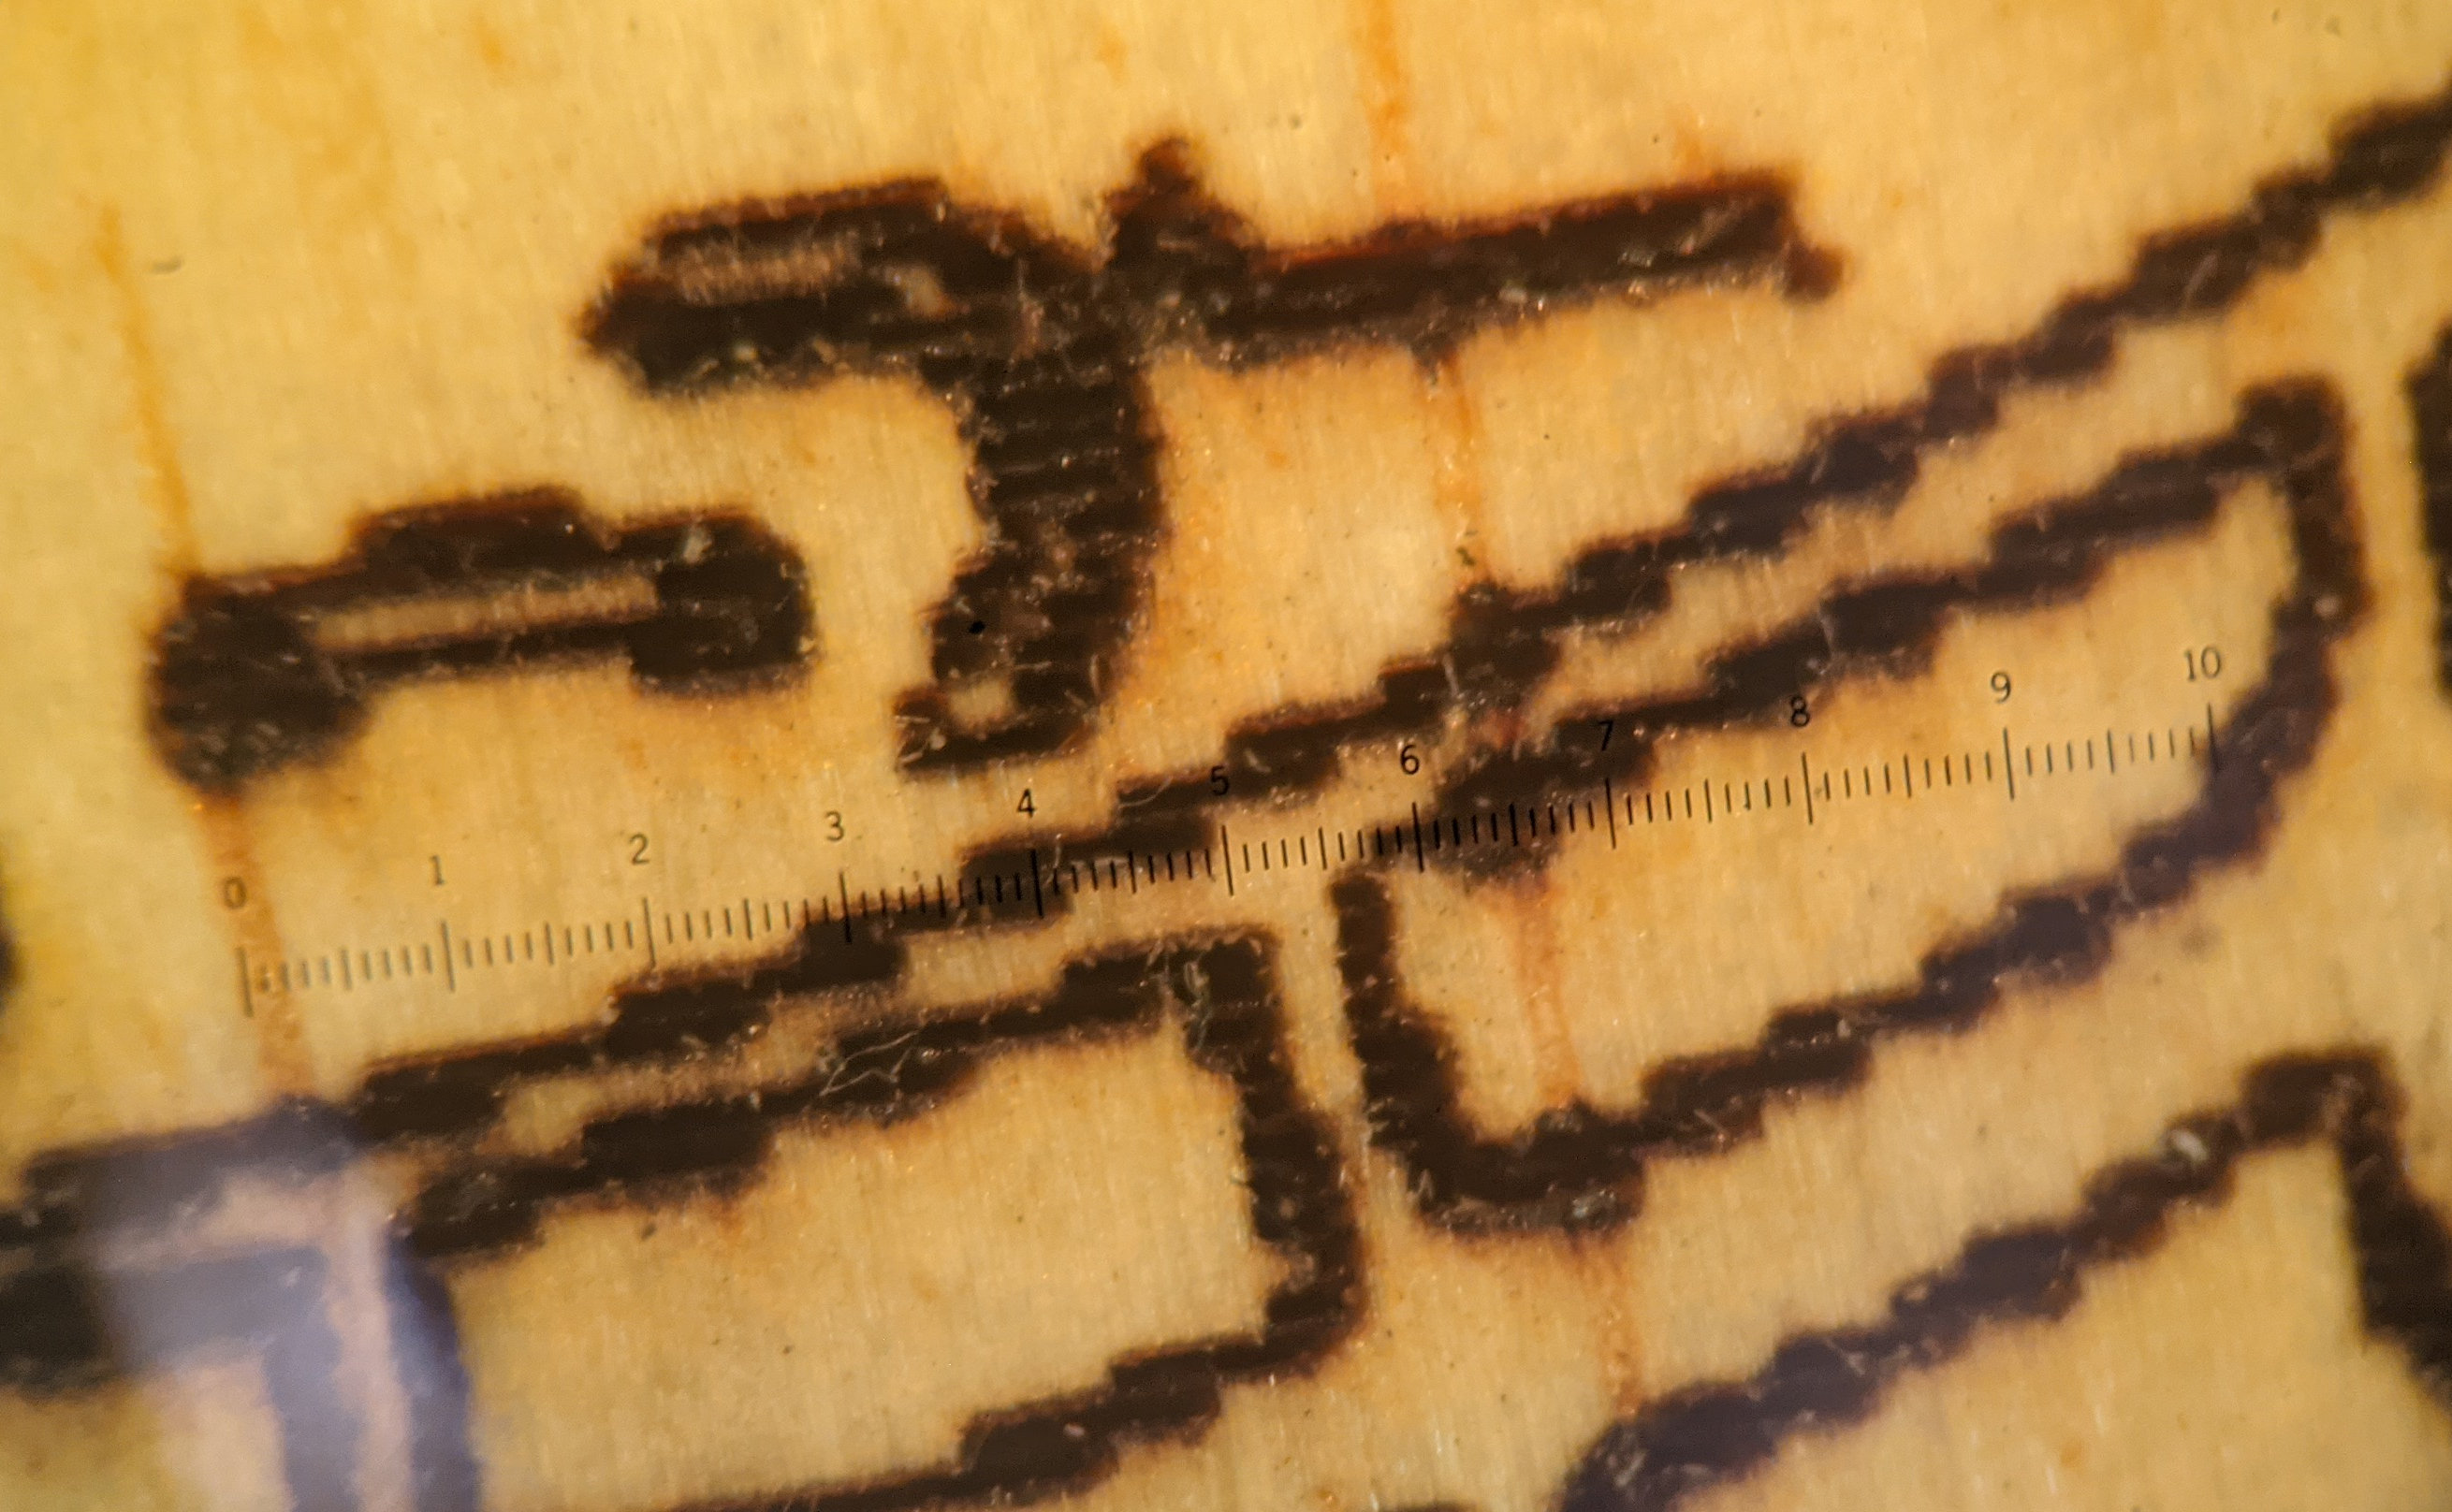
\includegraphics[width=0.8\textwidth]{burn-zoomed}
    \caption{Microscope image of trollface print}
    \label{fig:burn-zoomed}
  \end{center}
\end{figure}

A slight discrepancy was noticed in some instances, which were corrected in software.
In Figure \ref{fig:off-by-one} there can be seen a case where the burns would alternate
locations slightly when the direction was changed, and a case where the pixels were
spread too far apart.
\begin{figure}[H]
  \begin{center}
    
\includegraphics[width=0.4\textwidth]{test4}
    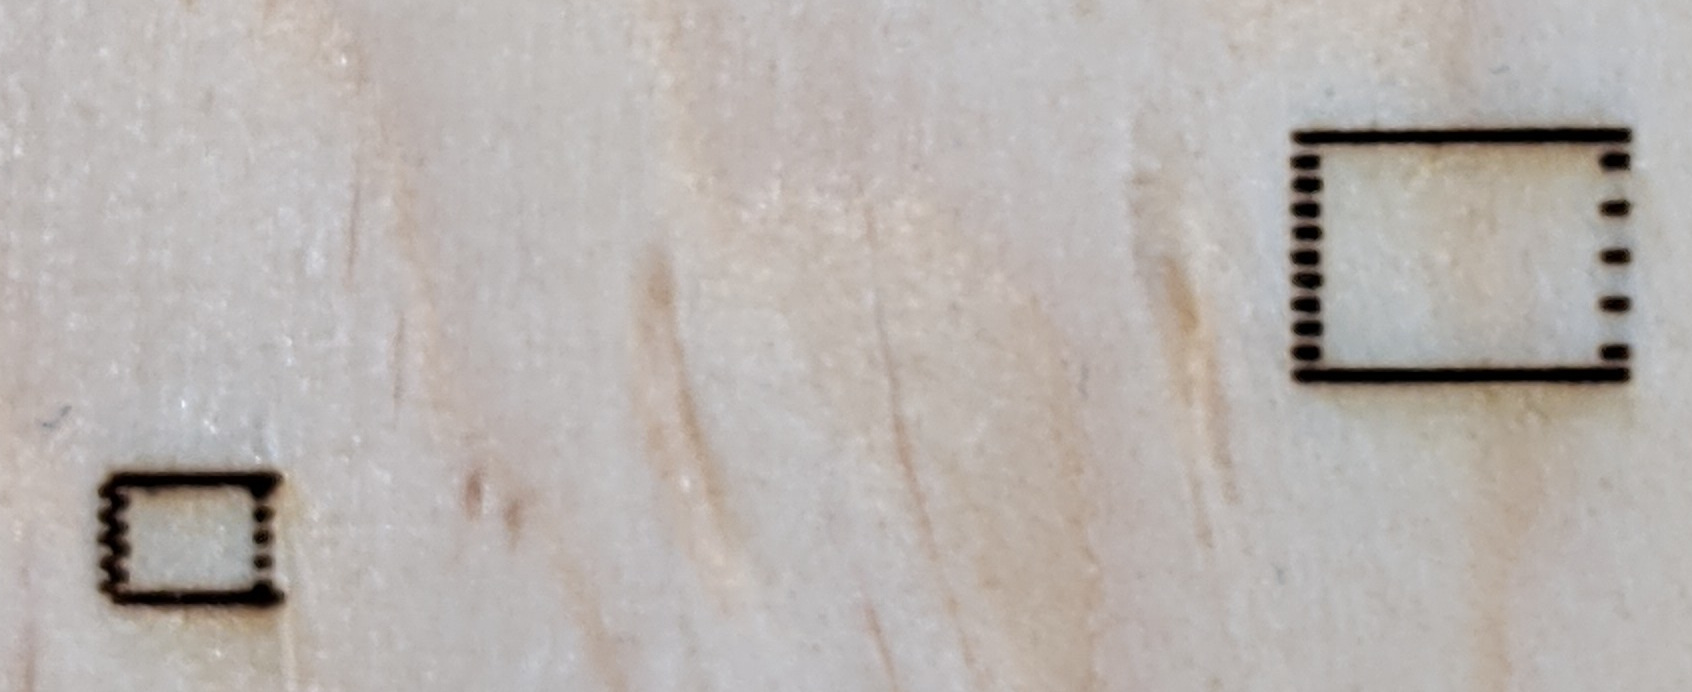
\includegraphics[width=0.4\textwidth]{burn-errors}
    \caption{The prepared input file and some erroneous outputs}
    \label{fig:off-by-one}
  \end{center}
\end{figure}

\section*{Appendices}
\subsection{Figures}

\end{document}
